\documentclass[a4paper,10pt]{ctexart}

\usepackage[utf8]{inputenc}
\usepackage[T1]{fontenc}
\usepackage{amsmath, amssymb, amsfonts}
\usepackage{graphicx}
\usepackage{booktabs}
\usepackage{lipsum}
\usepackage{multicol}
\usepackage{color,xcolor}
\usepackage{fancyhdr}
\usepackage{geometry}
\usepackage{tikz}
\usepackage{caption}
\usepackage{colortbl}

\geometry{margin=1.5cm}

\pagestyle{fancy}
\fancyhf{}
\lhead{打印机排版测试文档(彩色)}
\rhead{\today}
\cfoot{\thepage}

\title{彩色打印测试文档}
\author{测试用户}
\date{\today}

\begin{document}

\maketitle

\section*{字体与字号测试(含彩色)}

{\songti 宋体,正常字号。\par}
{\kaishu 楷体,用于说明文字。\par}
{\heiti 黑体,常用于标题。\par}

{\small 小号字体。Small font size.}
\par
{\normalsize 正常字号。Normal font size.}
\par
{\large 稍大字体。Large font size.}
\par
{\Large 更大字体。Larger font size.}
\par
{\huge 特大字体。Huge font size.}
\par
{\Huge 最大字体。HUGE font size.}

\bigskip

{\color{red} 红色文字},{\color{blue} 蓝色文字},{\color{green!70!black} 深绿色文字},{\color{orange} 橙色文字}。

中英文混排:This is a sentence with 中文夹杂其中 to test \textcolor{purple}{color and spacing}.

\section*{数学公式排版(含彩色)}

行内公式:设 $f(x) = \textcolor{blue}{\sin(x)}$,其导数为 $f'(x) = \textcolor{red}{\cos(x)}$。

\[
\textcolor{green!50!black}{\int_{-\infty}^{\infty} e^{-x^2} \, dx = \sqrt{\pi}}, \quad
\lim_{n \to \infty} \left(1 + \frac{1}{n}\right)^n = \textcolor{orange}{e}
\]

\section*{表格、图像与彩色填充}

\begin{minipage}{0.45\textwidth}
\centering
\captionof{table}{彩色背景表格}
\rowcolors{2}{gray!10}{white}
\begin{tabular}{cccc}
\toprule
序号 & 项目 & 数值 & 单位 \\
\midrule
1 & \textcolor{blue}{分辨率} & \textcolor{red}{600} & dpi \\
2 & \textcolor{green!60!black}{墨水类型} & 染料 & - \\
3 & 色彩模式 & \textcolor{purple}{CMYK} & - \\
\bottomrule
\end{tabular}
\end{minipage}
\hfill
\begin{minipage}{0.45\textwidth}
\centering
\captionof{figure}{图像与色带测试}
\includegraphics[width=0.9\linewidth]{example-image}

\vspace{0.5em}

\begin{tikzpicture}
\foreach \i/\c in {0/red, 1/orange, 2/yellow, 3/green, 4/blue, 5/purple} {
  \fill[\c] (\i,0) rectangle ++(1,0.4);
}
\end{tikzpicture}


\end{minipage}

\section*{灰阶渐变/模拟网点测试}

\begin{center}
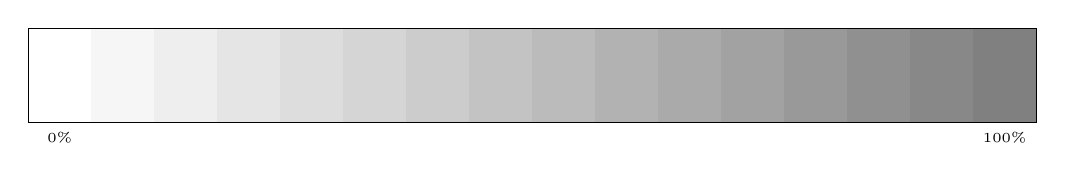
\begin{tikzpicture}
    \foreach \i in {0,...,15} {
        \fill[gray!\the\numexpr\i*100/15\relax] (\i*0.8,0) rectangle ++(0.8,1.2);
    }
    \draw[black] (0,0) rectangle (12.8,1.2);
    \node[below] at (0.4,0) {\tiny 0\%};
    \node[below] at (12.4,0) {\tiny 100\%};
\end{tikzpicture}
\end{center}

\noindent\textbf{模拟网点版本(低分辨率放大 + TikZ 网格遮罩):}

\begin{center}
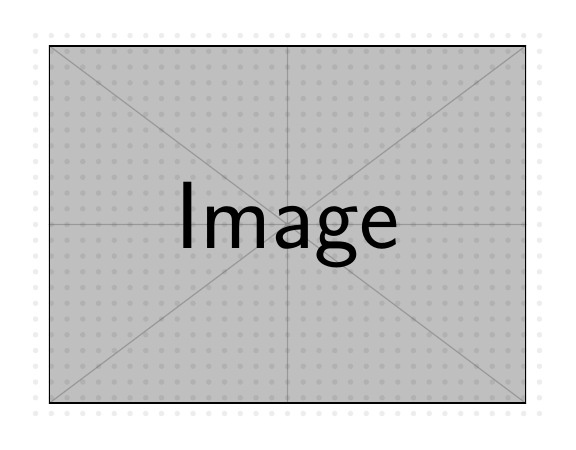
\begin{tikzpicture}
    \node[inner sep=0pt] at (0,0) {\includegraphics[width=0.5\linewidth]{example-image}};
    \begin{scope}
        \clip (-3.3,-2.5) rectangle (3.3,2.5);
        \foreach \x in {-6,-5.8,...,6} {
            \foreach \y in {-6,-5.8,...,6} {
                \fill[black,opacity=0.07] (\x,\y) circle(0.035);
            }
        }
    \end{scope}
\end{tikzpicture}
\end{center}
\section*{排版密度测试}

\begin{multicols}{3}
\lipsum[1-2]
\end{multicols}

\section*{字符与符号测试}

符号:$ \textcolor{blue}{\alpha}, \beta, \gamma, \sum, \int, \infty, \nabla $

引号:“中文双引号”,‘中文单引号’;"English quotes", 'single quotes'

括号测试:(),[],\{ \}。百分号:\% \quad 井号:\# \quad 下划线:\_ \quad 反斜杠:\textbackslash

\end{document}
